\documentclass{article}

\usepackage{graphicx}
\graphicspath{ {./images/} }

\usepackage{tikz}
\usetikzlibrary{positioning,chains,fit,shapes,calc}
\newcommand{\indsize}{}
\newcommand{\colind}[2]{\displaystyle\smash{\mathop{#1}^{\raisebox{.5\normalbaselineskip}{\indsize #2}}}}
\newcommand{\rowind}[1]{\mbox{\indsize #1}}


\begin{document}
        
%Header
\begin{flushleft}
    Evan Wilcox\\
    CS1200 Fall 2018\\
    Homework 7\\
    Due: Wednesday 12/5/18
\end{flushleft}
        
%Problems
\begin{enumerate}

    %1
    \item Either draw a graph with the specified properties
    or explain why no such graph exists.

    \begin{enumerate}
        %a
        \item This graph does not exist because the degree of the graph is odd.
        
        %b
        \item Graph with four vertices of degrees 1,2,3 and 4.
        \begin{center}
            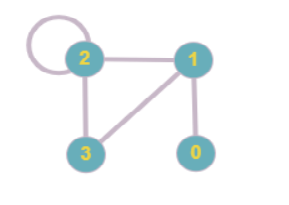
\includegraphics[scale=0.8]{1b}
        \end{center}

        %c
        \item Full binary tree with seven vertices.
        \begin{center}
            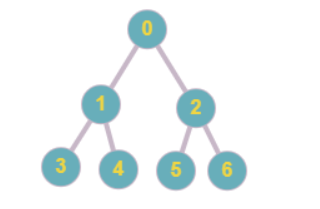
\includegraphics[scale=0.8]{1c}
        \end{center}
        
        %d
        \item This graph does not exist because the number of vertices - 1 equals the 
        number of edges.
        

    \end{enumerate}

    \vspace{2cm}
    %2
    \item 
    
    \begin{enumerate}
        %a
        \item  A Euler Circuit for the graph does not exist because at least one vertex has an 
        odd amount of connections.

        %b
        \item A Euler Circuit for the graph is 
        $v_{1}, v_{2}, v_{3}, v_{4}, v_{5}, v_{2}, v_{5}, v_{4}, v_{1}$.

        %c
        \item A walk for the graph is $A, B, D, E, A, D, C, A$.

        %d
        \item A Hamiltonian circuit for the graph is 
        $v_{0}, v_{7}, v_{6}, v_{2}, v_{5}, v_{4}, v_{3}, v_{1}, v_{0}$.
        
    \end{enumerate}
    
    \newpage
    %3
    \item 

    \begin{enumerate}
        %a
        \item  No there will be one person who can only shake two people hands.

        %b
        \item The height of the given binary tree is 6.

        %c
        \item Given the graph:

        \begin{enumerate}
            %i
            \item Find adjacency matrices.
            
            \begin{center}
                $\:\:\:B$
            \end{center}
            \[
                A \: \: \: \: \:
              \begin{array}{@{}c@{}}
                \rowind{1} \\ \rowind{2} \\ \rowind{3} \\ \rowind{4}
              \end{array}
              \mathop{\left[
              \begin{array}{ *{4}{c} }
                 \colind{0}{1}  &  \colind{0}{2}  &  \colind{1}{3}  & \colind{1}{4}\\
                 0 & 0 & 1 & 0\\
                 1 & 1 & 0 & 0\\
                 1 & 0 & 0 & 1\\
              \end{array}
              \right]}^{
              }
            \]
            
            %ii
            \item There are no distinct walks of length 2 from $v_{2}$ to $v_{3}$.
            
        \end{enumerate}
    \end{enumerate}

    \vspace{2cm}
    %4
    \item  Find a system of pipelines to connect all the cities and yet
    minimize the total cost by using Kruskal's algorithm (Show the work step by step).

    \begin{center}
    \begin{tabular}{ |c|c|c|c| }
        \hline
        \textbf{Iteration} & \textbf{Edge Considered} & \textbf{Weight} & \textbf{Action}\\
        \hline
        1 & Cheyenne, Denver & 0.8 & Added\\
        \hline
        2 & Albuquerque, Amarillo & 1.1 & Added\\
        \hline
        3 & Phoenix, Albuquerque & 1.2 & Added\\
        \hline
        4 & Salt Lake City, Cheyenne & 1.5 & Added\\
        \hline
        5 & Salt Lake City, Denver & 1.6 & Not Added\\
        \hline
        6 & Denver, Amarillo & 1.7 & Added\\
        \hline
    \end{tabular}

    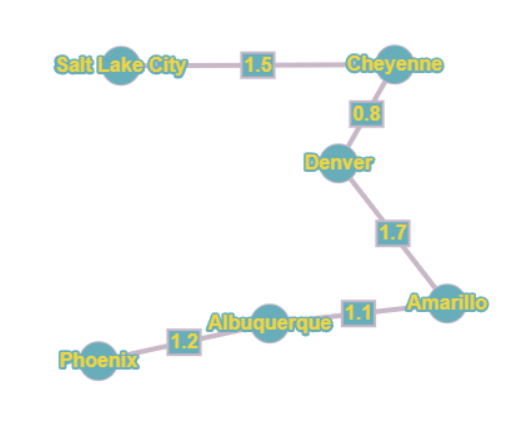
\includegraphics[scale=0.7]{4}
    \end{center}

    \newpage
    %5
    \item 
    
    \begin{enumerate}
        %a
        \item  If any seven digits could be used to form a telephone number, how many seven-digit
        telephone numbers would not have any repeated digits?
        $${10 \choose 7} = \frac{10!}{7!(3!)} = 120$$

        %b
        \item How many seven-digit telephone numbers would have at least one repeated digit?
        $$P(10, 7) - {10 \choose 7} = 604,800-120 = 604,680$$

        %c
        \item What is the probability that a randomly chosen seven-digit telephone number would
        have at least one repeated digit?
        $$\frac{P(10, 7) - {10 \choose 7}}{P(10, 7)} = \frac{604,680}{604,800} = 99.98\%$$
        
    \end{enumerate}

    \vspace{2cm}
    %6
    \item  Suppose that in a certain state, all automobile license plates have four upper case
    letters followed by three digits.

    \begin{enumerate}
        %a
        \item How many license plates could begin with M and end in 0?
        $$P(26, 3)*P(10, 2) = \frac{26!}{(26-3)!} * \frac{10!}{(10-2)!} = 15,600*90 = 1,404,000$$

        %b
        \item How many license plates are possible in which all the letters and digits are distinct?
        $${26 \choose 4}{10 \choose 3} = \frac{26!}{4!(22!)} * \frac{10!}{3!(7!)} = 14,950*120 = 1,794,000$$

        %c
        \item How many license plates could begin with MO and have all letters and digits distinct?
        $${24 \choose 2}{10 \choose 3} = \frac{26!}{2!(22!)} * \frac{10!}{3!(7!)} = 276*120 = 33,120$$

    \end{enumerate}
    
    \newpage
    %7
    \item A club is considering changing its bylaws. In an initial straw vote on the issue, 24
    of the 40 members of the club favored the change and 16 did not. A committee of six is
    to be chosen from the 40 club members to devote further study to the issue.

    \begin{enumerate}
        %a
        \item  How many committees of six can be formed from the club membership?
        $${40 \choose 6} = \frac{40!}{6!(36!)} = 3,838,380$$
        
        %b
        \item  How many of the committees will contain at least three club members who, in the
        preliminary survey, favored the change in the bylaws?
        $${24 \choose 3}{16 \choose 3} = \frac{24!}{3!(21!)} * \frac{16!}{3!(13!)} = 2,024*560=1,133,440$$
    
    \end{enumerate}
   
    \vspace{3cm}
    %8
    \item Write a program to calculate the binomial coefficients recursively.
    \begin{center}
        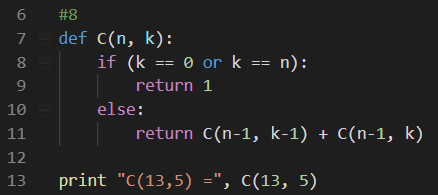
\includegraphics[scale=0.75]{8a}\\
        $$C(13, 5) = 1287$$.\\
        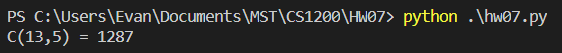
\includegraphics[scale=0.75]{8b}\\
    \end{center}

\end{enumerate}

\end{document}